\section{Experiments}
\label{sec:experiments}

\subsection{Benchmarks}
We evaluate PivotRL on the following agentic benchmarks:
\begin{itemize}
  \item \textbf{$\tau^2$-bench} \citep{barres2025tau2bench} focuses on conversational tool-use in a multi-turn customer service setting. It contains 3 subsets: Retail and Airline \citep{yao2024taubench}, which tests agent tool-calling, and Telecom, which adds the complexity of user tool-calls. We keep the user model fixed to \texttt{Qwen3-235B-A22B-Instruct-2507} across our evaluations.
  \item \textbf{Terminal-Bench} \citep{tbench_2025} evaluates the model on bash terminal-use tasks that range from filesystem navigation, coding, and system administration to complex problem-solving scenarios such as training machine learning models, configuring legacy systems, and reverse engineering binary files. We evaluate on the TBCore-v1.1 set of questions using the Terminus-2 harness.
  \item \textbf{Swe-Bench} \citep{jimenez2024swebench} evaluates the model on various real-world programming tasks that can be described as understanding an issue, localizing the issue in a codebase, and creating a code patch to resolve the issue. We use the SWE-Bench-Verified subset which is a widely adopted set of 500 verifiable questions.
  \item \textbf{BrowseComp}
  \citep{wei2025browsecompsimplechallengingbenchmark} is tests the search agent capabilities of a model through very difficult questions that require critical reasoning and the use of a search engine to answer correctly. It often results in very long trajectories with many search calls for each problem, and is shown to be a hard benchmark for current frontier LLMs.
\end{itemize}

\begin{table}[!t]
\centering
\small % Slightly smaller font to ensure it fits well in double-column layouts
\begin{tabular}{lcccc}
\toprule
\textbf{Benchmark} & Filtering & \textbf{Qwen3-30B (\%)} & \textbf{PivotRL (\%)} & \textbf{Gain ($\Delta$)} \\ 
\midrule
$\tau^2$-Bench             & $\mathcal{D}_{\text{adv}}$    & 44.35 & 63.81 & +19.46 \\
SWE-Verified               & $\mathcal{D}_{\text{adv}}$  & 19.07 & 30.80 & +11.73 \\
Terminal-Bench             & $\mathcal{D}_{\text{adv}}$  & 5.42  & 20.00 & +14.58 \\ 
BrowseComp                 & $\mathcal{D}_{\text{random}}$ & 2.50  & 11.30 & +8.80  \\
\bottomrule
\end{tabular}
\caption{Main results of benchmark accuracy gain after training with PivotRL on \texttt{Qwen3-30B-A3B-Thinking-2507}.}
\label{tab:main_results_enhanced}
\end{table}

\subsection{Main Results}
We conduct all PivotRL experiments on \texttt{Qwen3-30B-A3B-Thinking-2507}, using Nemo-RL \citep{nemo-rl} as the training framework and utilizing Nemo-Gym \citep{nemo-gym} for the environment rollouts. We show considerable gain in all four domains of Conversational Tool-Use, Software Engineering, Terminal Use, and Search using PivotRL as showed in Table \ref{tab:main_results_enhanced}. All four experiments were run independently of each other, with separate resulting policies. We discuss individual experiments and results below.

\begin{table*}[!bt]
\small
\centering
\setlength{\tabcolsep}{6pt}
% \begin{tabular}{l|c|c|c|c|c|c}
\newcolumntype{F}{>{\centering\arraybackslash}p{0.8cm}} % adjust 1.3cm to desired 
\newcolumntype{C}{>{\centering\arraybackslash}p{0.8cm}} % adjust 1.3cm to desired column width
\begin{tabular}{l|F|F|C|C}
\toprule
& \multicolumn{1}{c|}{\textbf{$\tau^2$-Airline}}
& \multicolumn{1}{c|}{\textbf{$\tau^2$-Retail}}
& \multicolumn{1}{c|}{\textbf{$\tau^2$-Telecom}}
& \multicolumn{1}{c}{\textbf{$\tau^2$-Average}} \\
\midrule
gpt-oss-120b-high
& 55.33 & 58.19 & 67.20 & 60.24 \\
gpt-oss-20b-high
& 43.33 & 50.20 & 52.63 & 48.72 \\
Qwen3-235B-A22B-Thinking-2507
& 50.0 & 66.08 & 46.78 & 54.29 \\
\midrule
Qwen3-30B-A3B-Thinking-2507
& 50.00
& 54.39
& 28.65
& 44.35 \\
\hdashline
Qwen + SFT
& 51.33
& 58.19
& 65.79
& 58.44 \\
Qwen + Random
& 58.00
& 63.74
& 57.31
& 59.68 \\
Qwen + All Mixed Rewards
& 61.33
& 66.08
& 56.73
& 61.38 \\
Qwen + Large Advantage Gap
& 58.67
& 69.01
& 63.74
& 63.81 \\
\bottomrule
\end{tabular}
\caption{Effect of pivot selection algorithm on downstream performance. Best checkpoint over training. While randomly choosing pivots improves the model, choosing only pivots with mixed rewards provides a superior learning signal, and further constraining the pivots to have mean reward $\leq 0.6$ yields the best set of pivot training dataset.}
\label{tab:results_tau_rl_pivot_selection}
\end{table*}

\subsection{$\tau^2$-bench}
\subsubsection{Experimental Details}
We curate an SFT training set consisting of $281774$ trajectories across $838$ domains by following a synthetic data generation procedure similar to ToolAce \citep{liu2025toolacewinningpointsllm}, Kimi-K2 \citep{kimiteam2025kimik2openagentic}, and DeepSeek-V3.2 \citep{deepseekai2025deepseekv32pushingfrontieropen}. We train on top of the \texttt{Qwen3-30B-A3B-Thinking-2507} \citep{qwen3technicalreport} model and compare with open-source models such as \texttt{Qwen3-235B-A22B-Thinking-2507} and the \texttt{gpt-oss} \citet{openai2025gptoss120bgptoss20bmodel} models under the high reasoning setting.

\subsubsection{Results}
Under the best pivot selection setting, our method is able to achieve higher overall accuracy in $\tau^2$-bench than using SFT, and outperform even much larger models such as the \texttt{Qwen-235B} and \texttt{oss-120B models}. Our results are summarized in Table \ref{tab:results_tau_rl_pivot_selection}. Both the SFT baseline and the RL results were chosen from the best checkpoint across a fixed training experiment.

% \begin{figure}[t]
%     \centering
%     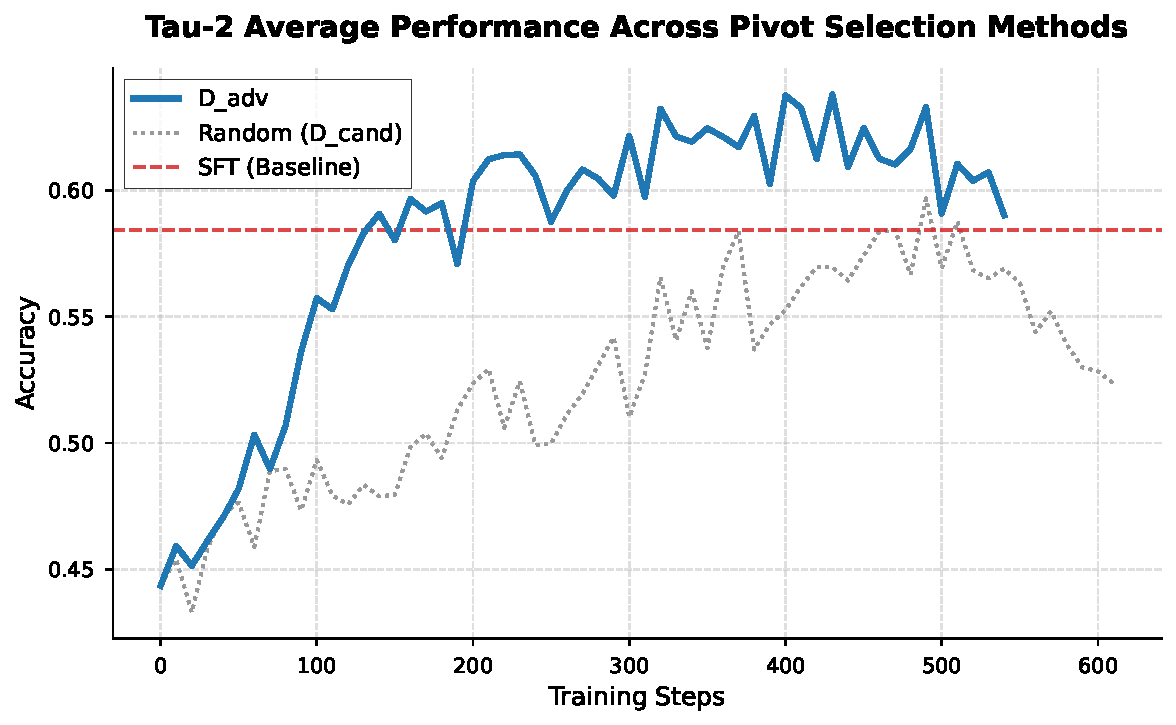
\includegraphics[width=0.5\textwidth]{figures/main_average_validation.pdf}
%     \caption{$\tau^2$-bench performance throughout RL training. Choosing pivots with a large advantage gap yields superior model improvement compared to choosing pivots with nonzero advantage or randomly choosing pivots.}
%     \label{fig:rl_tau_pivot_selection_acc}

%     \centering
%     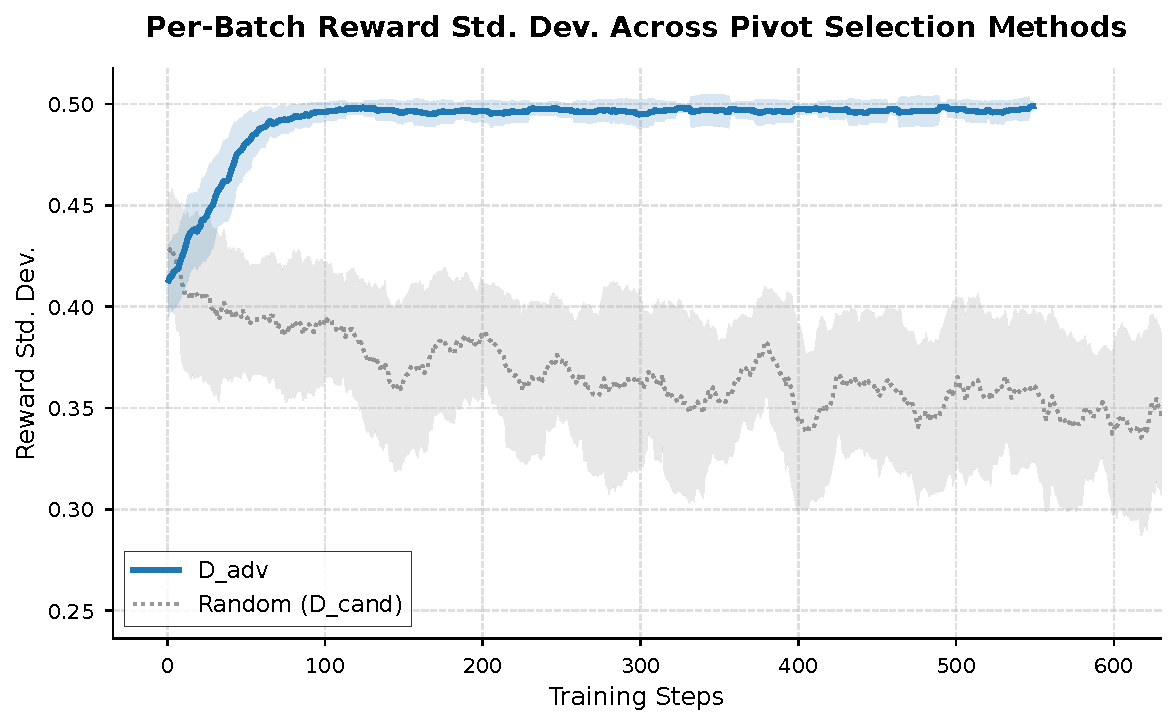
\includegraphics[width=0.5\textwidth]{figures/tau_reward_stddev.pdf}
%     \caption{$\tau^2$-bench training reward standard deviation over training. The random reward setting quickly yields unbalanced training rewards while the mixed rewards and high advantage gap settings leads to higher standard deviation in training rewards per group, allowing for better GRPO training.}
%     \label{fig:rl_tau_pivot_selection_acc}
% \end{figure}
\begin{figure}[t]
    \centering
    % Left side minipage
    \begin{minipage}{0.48\textwidth}
        \centering
        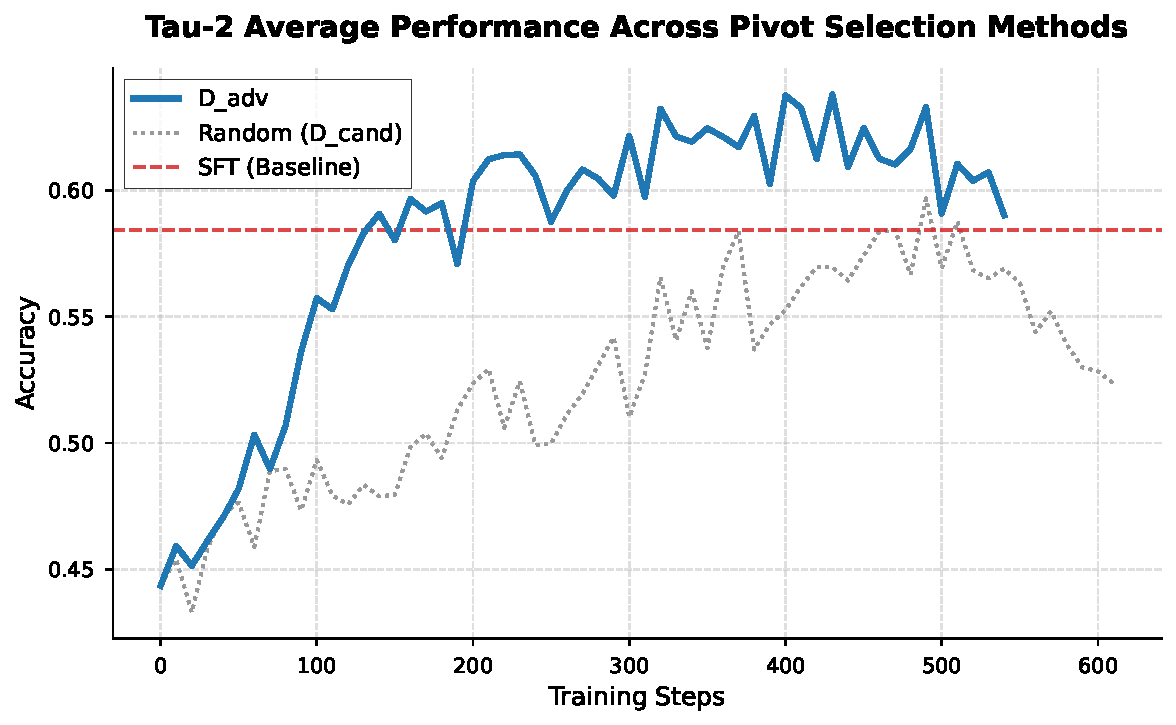
\includegraphics[width=\linewidth]{figures/main_average_validation.pdf}
        \caption{$\tau^2$-bench performance throughout RL training. Choosing pivots with a large advantage gap yields superior model improvement, outperforming even SFT on the base dataset.}
        \label{fig:rl_tau_pivot_selection_acc}
    \end{minipage}
    \hfill % Adds horizontal space between the two minipages
    % Right side minipage
    \begin{minipage}{0.48\textwidth}
        \centering
        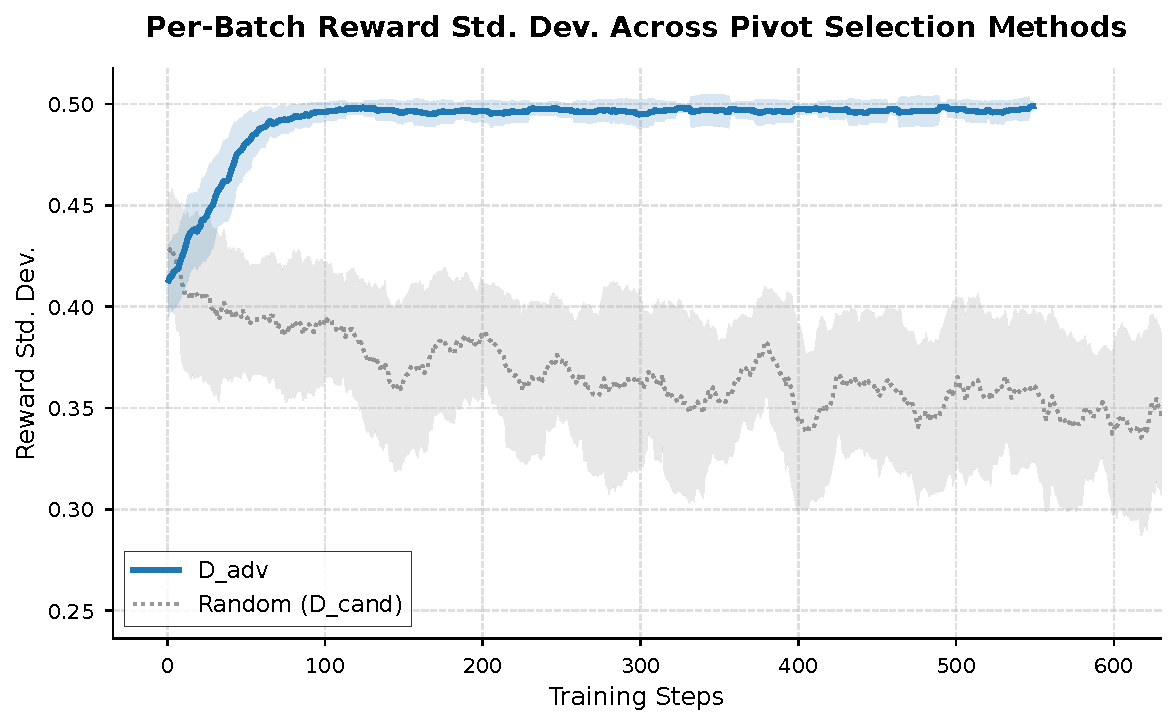
\includegraphics[width=\linewidth]{figures/tau_reward_stddev.pdf}
        \caption{$\tau^2$-bench training reward standard deviation. Higher standard deviation in training rewards allows for better GRPO training. Showing rolling standard deviation for viewer readability.}
        \label{fig:rl_tau_reward_stddev}
    \end{minipage}
\end{figure}

\begin{figure*}[t]
    \centering
    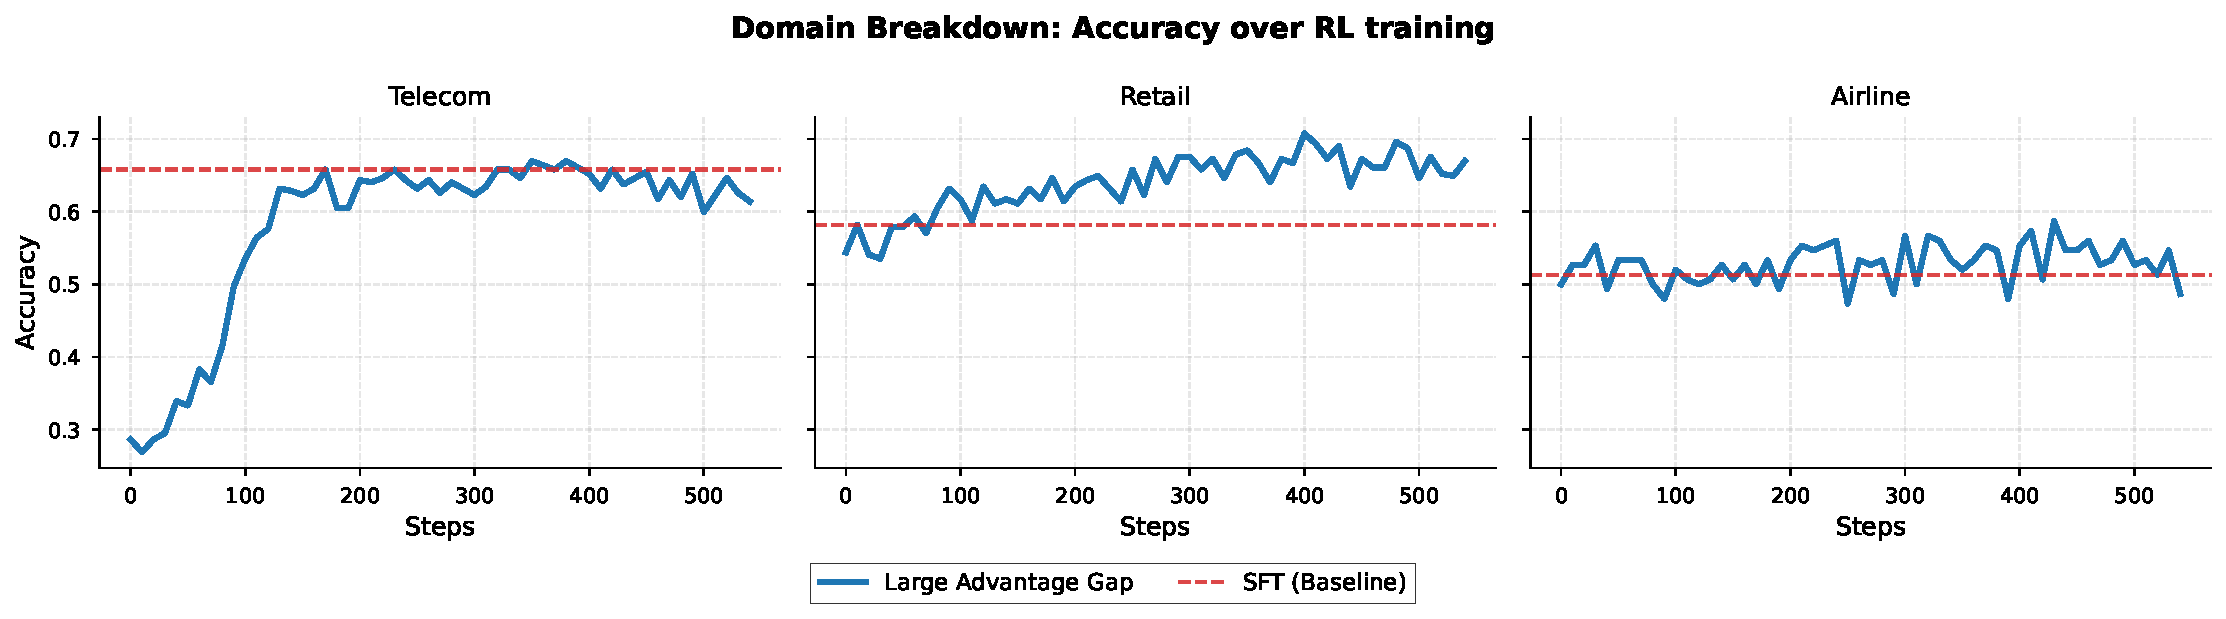
\includegraphics[width=1.0\textwidth]{figures/main_per_domain_validation_difficulty.pdf}
    \caption{Per-domain benchmark performance over RL training. From left to right: Telecom, Retail, Airline.}
    \label{fig:rl_domain}
\end{figure*}

\begin{table}[t]
\small
\centering
\setlength{\tabcolsep}{6pt}
\begin{tabular}{lcc}
\toprule
& \textbf{$\tau^2$-Average} & \textbf{AIME 2025} \\
\midrule
Qwen3-30B-A3B-Thinking-2507 & 44.35 & 85.00 \\
\midrule
Qwen + SFT                  & 58.44 & 77.71 \\
Qwen + RL (Ours)            & 63.81 & 85.21 \\
\bottomrule
\end{tabular}
\caption{Effects of SFT vs RL on out-of-domain generalization.}
\label{table:results_tau_aime}
\end{table}

\subsubsection{Effect of Pivot Selection and Generalization Analysis}
In Figures \ref{fig:rl_tau_pivot_selection_acc} and \ref{fig:rl_tau_reward_stddev}, we observe the effect of different pivot selection algorithms by the change in accuracy over RL training steps as well as the training reward standard deviation over RL steps. While the random pivot selection baseline is able to improve the model, it under-performs the mixed rewards setting where at the beginning of training every input prompt has non-zero advantage. Empirically, this is shown as the standard deviation of the reward for that prompt across the rollouts being larger. Meanwhile, further constraining the dataset to choose from points where the advantage gap is large yields the best performing training dataset, improving the model accuracy from $44.35\%$ to $63.81\%$ after 430 steps of training. We also see that as training goes, the large advantage gap set also has a more balanced reward distribution for each prompt as can be seen with the higher training reward standard deviation.

In addition to in-domain improvement, our method also shows no degradation in other capabilities when compared to SFT. In Table \ref{table:results_tau_aime}, we show that starting from the original AIME 2025 accuracy of $85\%$, the SFT model degrades the accuracy of the model to $77.71\%$, while our RL model shows no regression to $85.21\%$. This is in line with observations across the field that SFT is susceptible to catastrophic forgetting compared to RL \citep{shenfeld2025rlsrazoronlinereinforcement, chen2025retainingdoingroleonpolicy, lu2025onpolicydistillation}, and opens a possibility of directly replacing SFT stage with our method in model training.


\subsection{Terminal-Bench}
\subsubsection{Experimental Details}
We collected resolved and completed trajectories from \texttt{Qwen/Qwen3-Coder-480B-A35B-Instruct} and \texttt{moonshotai/Kimi-K2-Instruct} on Terminal Bench using the Terminus 1 and Terminus 2 agents, and use all assistant bash actions as pivots. From the $\mathcal{D}_{\text{adv}}$ setting, we additionally deduplicate similar commands to achieve diversity in the data. Our final training set consisted of approximately 20,000 samples. For verification in the RL environment, we employed output schema validation, string similarity, and equivalency-based LLM-as-judge in the reward design.

\begin{table}[t]
\small
\centering
\setlength{\tabcolsep}{6pt}
\begin{tabular}{lcc}
\toprule
& \textbf{Terminal Bench} & \textbf{AIME 2025} \\
\midrule
Qwen3-30B-A3B-Thinking-2507 & 5.42 & 85.00 \\
\midrule
Qwen + SFT                  & 13.75 & 10.42 \\
Qwen + RL (Ours)            & 20.00 & 82.08 \\
\bottomrule
\end{tabular}
\caption{Terminal-Bench and AIME 2025 results.}
\label{table:results_terminal}
\end{table}

\subsection{SWE-Bench Verified}
\subsubsection{Experimental Details}
We use an internal dataset of trajectories generated using the OpenHands \citep{wang2025openhandsopenplatformai} and SWE-Agent \citep{yang2024sweagentagentcomputerinterfacesenable} harnesses on tasks from SWE-Gym \citep{pan2025trainingsoftwareengineeringagents} using the \texttt{Qwen/Qwen3-Coder-480B-A35B-Instruct} \citep{qwen3technicalreport} model. We evaluate the mean@3 score using the OpenHands harness. \\
To create the PivotRL dataset, we use all tool call actions as pivots. We curate a final dataset of $15204$ prompts with mixed rewards for training. As there is 


\subsection{BrowseComp}
\subsubsection{Experimental Details}
To use a private search agent focused SFT dataset with trajectories generated from \texttt{DeepSeek-V3.2} that utilizes an online search engine to answer multi-hop questions. We curate a set of $13215$ samples and use random filtering ($\mathcal{D}_{\text{random}}$) due to the small size of the dataset. We are able to improve \texttt{Qwen3-30B-A3B-Thinking-2507} from $2.5$ accuracy to $11.3$.